\section{Partie graphique}


\subsection{Coté interface utilisateur}
\subsubsection{MaterializeCSS}
Pour l'interface utilisateur, nous avons dû utiliser la bibliothèque graphique \href{http://www.materializecss.com/}{{\tt MaterializeCSS}} qui fournit un dossier compressé comprenant tous les fichiers de base d'un site web. Ceci permet d'avoir une architecture de fichiers déjà existante et fournir les fichiers CSS nécessaires pour avoir un visuel optimisé et un design attirant.

Ainsi, il suffit d'appeler un élément graphique de HTML, de lui donner la classe correspondante implémentée dans MaterializeCSS et le visuel est prêt.

%%
\subsubsection{Structure du site}

Le site est en {\tt monopage}, c'est à dire qu'il n'y a pas de présence de plusieurs fichiers HTML à charger ou d'un serveur avec une base de données pour les différents élements.

Pour passer d'un contenu à un autre, nous utilisons l'élément HTML de "navigation". Ainsi, cela donne l'effet de trois pages: "Acceuil", "Commencer" et "A Propos" alors qu'il ne s'agit que d'un seul fichier HTML.\\

Dans la partie "Commencer", nous pouvons séparer cette partie en trois sous-catégories. La première permet à l'utilisateur de saisir ces paramètres (les fichiers de données, ses fonctions map/reduce et les paramètres du cluster).
La seconde permet soit d'écrire les fonctions map/reduce directement sur le site, ou de visualiser le code fournis pour le corriger directement.
Enfin la dernière section concerne la simulation avec FATuM pour le cluster et une colonne à droite de la page pour l'affichage des données contenues dans un slot.

\subsubsection{Les Loaders}
\begin{figure}[H]
  \centering
    
\includegraphics[scale=0.5]{images/loader.png}
        \caption{Loader}
\end{figure}
Le temps de chargement du site au démarrage ainsi que lors du lancement de la simulation sont long. Cette lenteur peut être interpréter comme un mauvais chargement des données par l'utilisateur. C'est pourquoi notre objectif était de rajouter un "loader" (voir Figure 4.1) au démarrage de la page pour signifier le chargement de FATuM et un autre pour le temps de calcul de la simulation. Le loader du démarrage fonctionne, malheureusement, celui de la simulation n'a pas pu être implémenter. En effet, le site se bloque le temps de calcul ce qui empêche l'utilisation du loader.

\subsubsection{Les paramètres}
Les {\tt paramètres} données par l'utilisateur doivent remplir certaines conditions.
\begin{itemize}
\item Le cluster du Map doit au grand maximum contenir entre 1 et 20 pc et entre 1 et 24 coeur . \\ Cette limitation est visuelle car au delà, la lisibilité n'est plus assuré. Il s'agit là, d'un choix suite aux conseils du client.
\item Le cluster de Reduce doit être comprise entre 1 et le nombre de slots total du cluster de Map.
\item Le fichier js des fonctions map/reduce n'étant pas nécessaire pour l'utilisation car nous avons fournit un exemple de code dans "section  code" qui est utilisé pour la suite de l'application.
\item Le fichier csv doit être impérativement fournit et contenir des données.
Si l'utilisateur rafraîchit la page, cette variable disparaît, il faut donc la charger de nouveau.
\end{itemize}


\subsection{Simulation graphique(Fatum)}
Comme demandé par le client, nous avons utilisé la bibliothèque graphique \href{http://www.labri.fr/perso/aperrot/fatum/index.html}{{\tt FATuM}} développée au \href{http://www.labri.fr/}{{\tt LABRI}}. Cette bibliothèque permet d'afficher la simulation du cluster (voir Figure 4.2) avec différents composants graphiques et ne peut être utiliser pour l'interface utilisateur contrairement à MaterializeCSS.
%image fatum simple avec connection.
\begin{figure}[H]
  \centering
    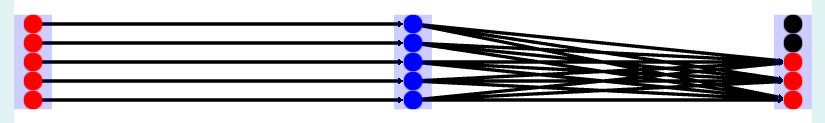
\includegraphics[scale=0.5]{images/graphiqueExemple.png}
        \caption{FATuM - Simulation}
\end{figure}

Nous utilisons plusieurs composants de FATuM:
\begin{itemize}
\item Les Marks
\item Les Connections
\item Le zoom
\item Une partie de la gestion d'un "clic souris"\\
\end{itemize}

\begin{figure}[H]
  \centering
    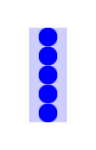
\includegraphics[scale=0.5]{images/marks.png}
        \caption{FATuM : Marks}
\end{figure}
Un {\tt Mark} (comme dans la figure ci-dessus) est un élément sous forme de cercle qui représente un slot du cluster. Ils sont séparés entre eux lorsque la limite de slots par PC est atteinte. Ainsi, chaque PC sont séparés graphiquement. Ces éléments graphiques sont dépendants des données fournies par l'utilisateur.\\

Les {\tt connections} sont les flèches qui vont d'un Mark vers un autre. Ils représentent le transfert de données entre les slots. On trouve des connections entre l'input de map et map ainsi que des connections entre map et reduce.\\

Le {\tt zoom} permet (si l'on pose le pointeur de la souris dans la zone de simulation gérée par FATuM) la gestion de la molette de la souris. Ainsi, en cas d'un gros cluster, l'ensemble reste lisible grâce à ce zoom. \\

Enfin, la gestion du {\tt "clic souris"}. Lors d'un clic dans la zone de simulation FATuM, les coordonnées récupérées sont celles de la fenêtre. Elles n'ont donc rien à voir avec celles de FATuM. La fonction {\tt windowToModel} nous a permis de transformer les coordonnées du clic en coordonnées compréhensibles par FATuM pour pouvoir exécuter le traitement suivant la zone de clic.


\subsubsection{Précision sur la fonction "search\_mark"}

\begin{lstlisting}
function search_mark(x, id) {
    var header_data, tmp_header;
    //type of the mark
    switch (x) {
        case indice_fatum_1:
            tmp_header = "Map Input--";
            break;

        case indice_fatum_2:
            tmp_header = "Map Output--";
            break;

        case indice_fatum_3:
            tmp_header = "Reduce Output--";
            break;
        default:
            return false;
    }
    var min = nb_slot + gap;
    var max = min + nb_slot;
    //researh the true id without the gap
    for (var i = 0; i < nb_pc; i++) {
        if (0 <= id && id < nb_slot) {
            header_data = "Slot " + id + ": --"; //exple: Slot 1: --Map Task--
            print_data(x, id, header_data + tmp_header);
            break;
        } else
        if (min <= id) {
            if (id < max) {
                id = id - (gap * (i + 1));
                header_data = "Slot " + id + ": --";
                print_data(x, id, header_data + tmp_header);
                break;
            }
        }
        min = max + gap;
        max = min + nb_slot;
    }
}
\end{lstlisting}

Cette fonction est particulière nécessite des précisions. 

En effet, pour différencier les blocs de pc, nous avons décider de mettre un décalage (variable gap) entre ces blocs. Ce décalage créer des erreurs d'id de mark par la suite. En effet, lorsque l'on clique sur un slot, sont id correspond à sa position dans l'axe y. Mais a cause de ce décalage, l'espacement était également considérer comme un bloc et les id était décaler.\\

D'autre part, cette fonction permet également de détecter quelle type de donnée on souhaite afficher. Pour cela, on utilise l'axe des x pour se repérer.

\subsubsection{La sortie console}

\begin{figure}[H]
  \centering
    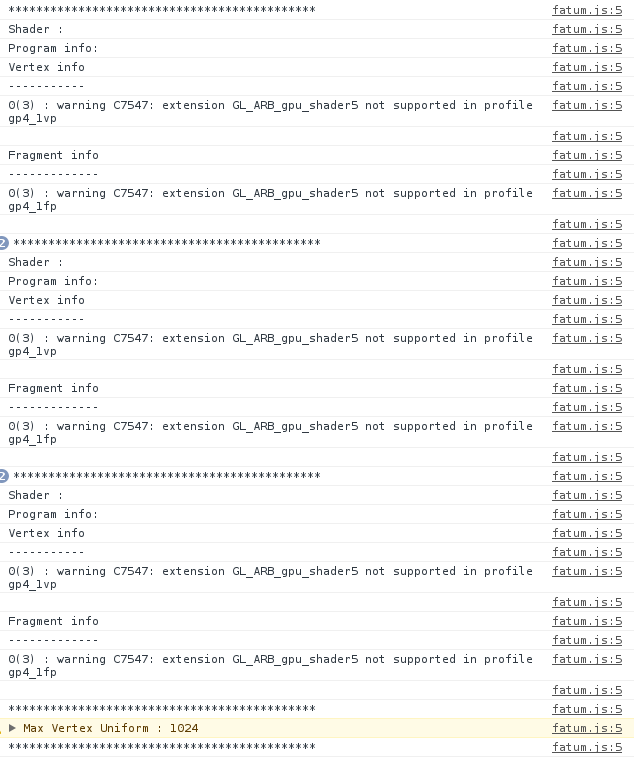
\includegraphics[scale=0.5]{images/console_fatum.png}
        \caption{Sortie console au démarrage}
\end{figure}
Lors du démarrage de l'application, l'initialisation de FATuM se fait, il est donc normal de voir en console (voir Figure 4.4), des informations concernant la bibliothèque.

\subsection{Difficulté lié à l'affichage}
Nos difficultés se sont principalement portées du fait que nous étions des débutants en web. Ainsi lorsqu'il a fallu utiliser la bibliothèque FATuM, les documentations n'étaient pas évidentes à comprendre au début. Surtout du fait que nous avions des exemples d'implémentation de FATuM dans une ancienne version de la documentation qui nous était fort utile pour comprendre les fonctions mais qui n'existaient plus pour certaines dans la nouvelle implémentation de FATuM.\\ 

Dans la nouvelle version de la documentation, il n'y a que les énoncés des fonctions, et c'est avec le temps que nous avons pris l'habitude de voir les exemples d'implémentation de FATuM dans l'ancienne documentation puis nous référer à la nouvelle documentation pour voir ce qui a changé.\\

\subsection{Amélioration possible}
Plusieur éléments peuvent être rajouté à la partie graphique pour améliorer l'utilisation de l'utilisateur et que nous n'avons pas pu implémenter
\begin{itemize}
\item le scrolling horizontal des données
\item un loader pour la simulation
\item Une optimisation visuelle du cluster
\end{itemize}


\paragraph{}
Concernant la partie visualisation, nous avons pensé que, plutôt que de rendre le cluster linéaire, c'est à dire: entrée Map puis sortie Map puis sortie Reduce chacun en ligne, le rendre cyclique.

\begin{figure}[H]
  \centering
    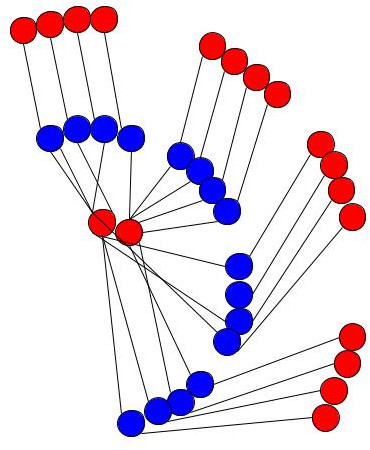
\includegraphics[scale=0.5]{images/cyclique.jpg}
        \caption{Exemple d'affichage}
\end{figure}
Ainsi, un très gros cluster serait plus ludique et plus compréhensible mais pourrait créer deux problèmes: il n'y a plus la linéarité du map reduce comme indiqué dans la littérature et les connections de fatum sont moins lisibles car elles vont traversé les marks intérieur.\\

Enfin, il y existe un conflit avec webGL. Nous ignorons à quoi ce bug est dû mais, il arrive que le navigateur ait des soucis avec cette bibliothèque. Ce problème peut être lié au cache. Mais nous n'avons pas de solution à proposer
